\section{Composición de la excavadora}

Voy a dividir cada una de las partes en subsecciones a continuación:

\subsection{Oruga}

La oruga la he modelado utilizando un cubo alargado y dos cilindros en los extremos con el mismo radio que la altura de los cubos, de manera que dé la sensación de oruga.

% foto de la oruga y la composicion (o no)
\begin{figure}[H]
   \centering
   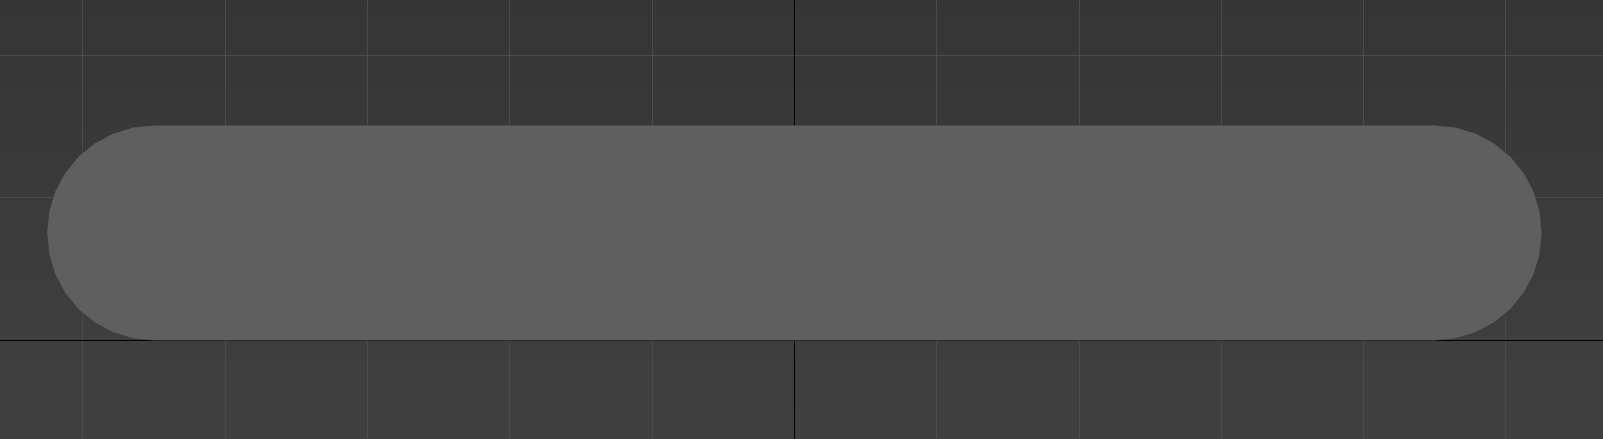
\includegraphics[width=0.5\textwidth]{imagenes/oruga.png}
   \caption{Forma final de la oruga.}
\end{figure}

\newpage

\subsection{Cabina}

La cabina está formada por 4 cubos: Uno primero para realizar la base sobre la que va a girar la propia cabina, otro donde se pondrá lo demás, uno atrás para hacer el compartimento del motor y uno último para hacer la ventana del conductor.

% foto de la forma final
\begin{figure}[H]
   \centering
   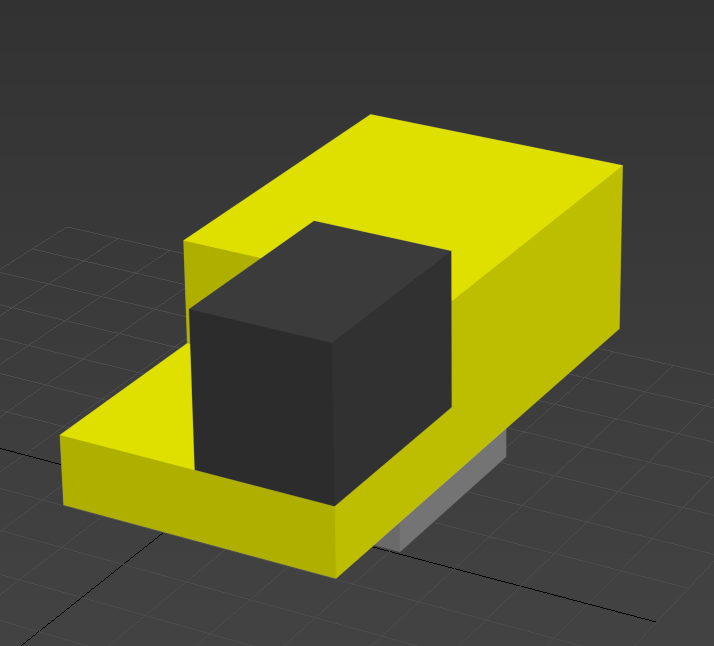
\includegraphics[width=0.5\textwidth]{imagenes/cabina.png}
   \caption{Forma final de la cabina, Se puede ver debajo como está la base sobre la que rota.}
\end{figure}

\subsection{Brazo}

El brazo lo he realizado utilizando dos cubos alargados para cada extremidad. Mientras que la pala la he modelado utilizando un cilindro de base triangular escalado en uno de sus lados, para que sea más similar a la realidad.

% foto del brazo
\begin{figure}[H]
   \centering
   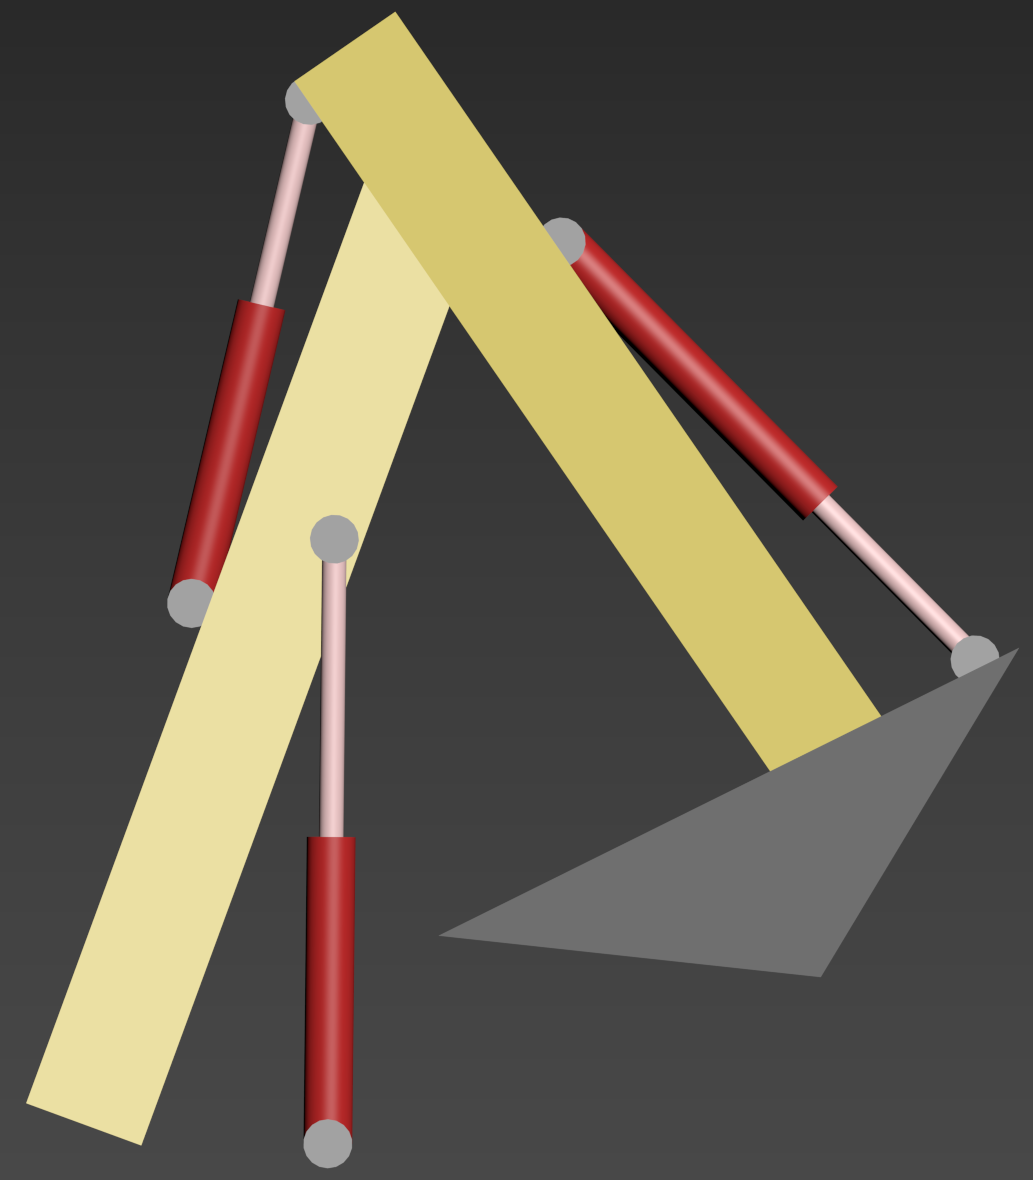
\includegraphics[width=0.5\textwidth]{imagenes/brazo.png}
   \caption{Forma final de brazo, junto con sus pistones hidráulicos.}
\end{figure}

Cabe destacar que he añadido pistones hidráulicos a las secciones del brazo para que sea más realista. Los pistones se modelan de la misma forma que en el seminario, con la única diferencia que los puntos de apoyo tienen un \textit{Link Position} para que se mantengan siempre pegados al brazo.

% foto del pistón
\begin{figure}[H]
    \centering
    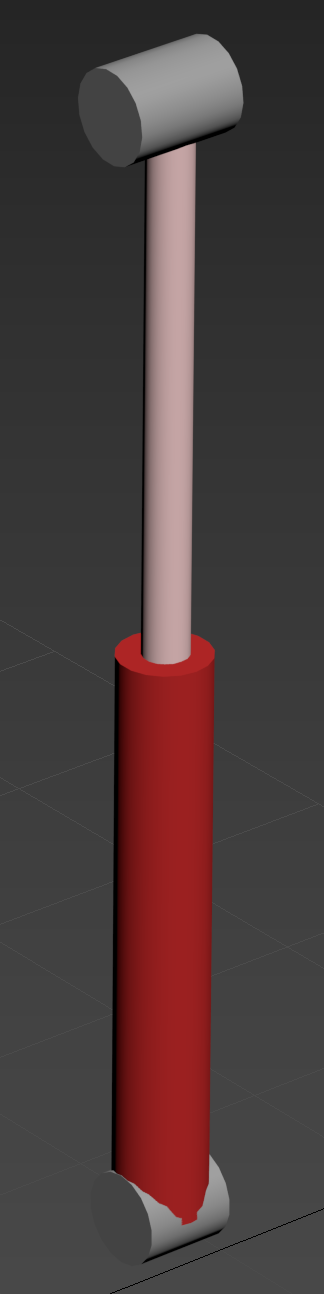
\includegraphics[width=0.1\textwidth]{imagenes/piston.png}
    \caption{Ejemplo del pistón hidráulico utilizado para el brazo.}
 \end{figure}